\section{Klienten}
\label{Technical_Client}
\subsection*{Arkitektur}
\label{Technical_Client_Archi}
Vi har implementeret vores klient med en \textit{Model-View-ViewModel}\footnote{http://msdn.microsoft.com/en-us/magazine/dd419663.aspx} (\textit{MVVM}) arkitektur. Klassisk \textit{MVVM} bruger et \textit{ViewModel} lag til at separere modellen og brugergrænsefladen. \textit{ViewModel} laget skal fungere som oversætter for brugergrænsefladen og modellen, således at der ingen kontakt er mellem dem. 

I vores implementering har hvert \textit{View} en \textit{ViewModel}, som laver det meste af logikken (opdatering af gitrene, konstruktion af nye booking objekter, m.m.). \textit{View}s styrer selv, hvad der skal kaldes på dens tilhørende \textit{ViewModel} ved forskellige events.

Normalt er modellen i \textit{MVVM} en database, men da vi anvender det i forbindelse med en service, bruger vi service interfacet som model i stedet for vores database. Dette betyder i realiteten, at modellen bliver delt op i fire lag, hvis man ser den som en helhed (klient model, service interface, logik til databasekald og databasen selv). Hvis vi ikke havde lavet en service, ville man kunne have reduceret dette til et eller to lag, og dermed er mængden af nødvendig kode langt mindre.

Vi har desværre ikke opfyldt vores mål om at have en \textit{MVVM} arkitektur i den grad, som vi ønskede. Figur \ref{Fig:Technical_Client_Archi_nsd} illustrerer afhængigheder for vores namespaces i klienten. Hvis \textit{MVVM} arkitekturen skulle være opfyldt i helhed, ville hverken \textit{GUI} eller \textit{ViewModel} være afhængig af \textit{BookItService}.

\begin{figure}[h!]
  \centering
    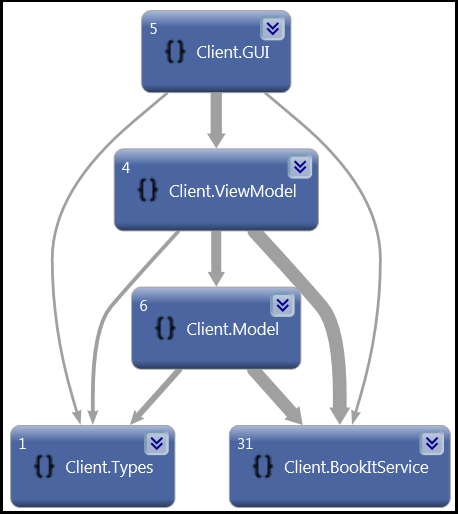
\includegraphics[width=0.4\textwidth]{Chapters/Design/Technical/Images/NamespaceDependencies}
  \caption{De forskellige lag i klienten og deres afhængigheder.}
\label{Fig:Technical_Client_Archi_nsd}
\end{figure}

\subsection*{Implementering af brugergrænsefladen}
\label{Technical_Client_GUI}
Klientens brugergrænseflade er udviklet i ASP.net\footnote{http://www.asp.net/} Web Forms og er kodet i C\#. Vi kalder vores brugergrænseflade for "klienten", selvom den er hostet serverside. Dette gør vi, fordi det er en "klient" til vores system. Vores klient skal stadig hostes af en server, som udfører det meste af klientens funktionalitet.

 Vores \textit{View}s består af .apsx filer, som beskriver udseendet af vores brugergrænseflade. Hvert \textit{View} har desuden en code-behind fil, som beskriver funktionaliteten af knapper og andre elementer på siden. Desuden har vi en \textit{Master Page}, som sørger for, at vi anvender et konsistent design.
\\Derudover anvender vi Cascading Style Sheets til at hjælpe med det konsistente design og Javascript til funktionalitet, som skal udføres af brugerens browser i stedet for serveren, som hoster klienten.